\documentclass[border=0.05cm]{standalone}
\usepackage{tikz}
\usepackage{xcolor}
\usetikzlibrary{automata, arrows.meta, positioning}
\usepackage{fontspec}
\setmainfont{Arial}
\usepackage{amsmath}

% Define colors based on split-complementary scheme
% https://copic.too.com/blogs/educational/analogous-complimentary-and-split-complementary-color-schemes?srsltid=AfmBOoqZ8Nt71usioxMxPyKzjQ5vDcxs2B_imasd_wZa50UB5cZX6xCL
\definecolor{dftcolor}{RGB}{44, 163, 207}  
\definecolor{simcolor}{RGB}{237, 156, 44} 
\definecolor{expcolor}{RGB}{222, 70, 28}

% Define styles
\tikzset{
	%dft/.style={draw=dftcolor!80!black, fill=dftcolor!40, minimum size=2cm},
	%simulated/.style={draw=simcolor!80!black, fill=simcolor!30, minimum size=2cm},
	%experimental/.style={draw=expcolor!80!black, fill=expcolor!40, minimum size=2cm},
    dft/.style={draw=dftcolor!80!black, fill=dftcolor!40, shape=rectangle, minimum width=2cm, minimum height=2cm, rounded corners=12pt},
	simulated/.style={draw=simcolor!80!black, fill=simcolor!30, shape=rectangle, minimum width=2cm, minimum height=2cm, rounded corners=12pt},
	experimental/.style={draw=expcolor!80!black, fill=expcolor!40, shape=rectangle, minimum width=2cm, minimum height=2cm, rounded corners=12pt},
	MU/.style={->, line width=1.2pt, color=simcolor},
	UM/.style={thick, ->, color=dftcolor},
	UV/.style={->,  line width=1.2pt, color=expcolor},
	VU/.style={thick, ->, color=simcolor},
	VM/.style={->, line width=1.2pt, color=dftcolor},
	annotation/.style={font=\small}
}

\begin{document}
	
	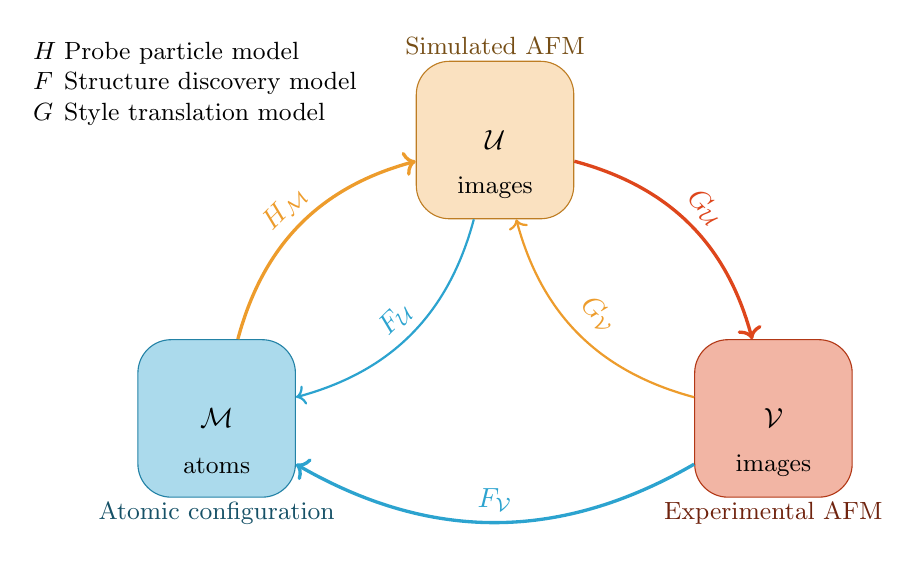
\begin{tikzpicture}[node distance = 5cm, on grid, auto]
		
		% Nodes
		\node (M) [state, dft] {$\mathcal{M}$};
		\node (U) [state, above right = of M, simulated] {$\mathcal{U}$};
		\node (V) [state, below right = of U, experimental] {$\mathcal{V}$};
		
		% Annotations
		\node[below=1.2cm of M, annotation, text=dftcolor!50!black] {Atomic configuration};
		\node[below=0.6cm of M, annotation] {atoms};
		
		\node[above=1.2cm of U, annotation, text=simcolor!50!black] {Simulated AFM};
		\node[below=0.6cm of U, annotation] {images};
		
		\node[below=1.2cm of V, annotation, text=expcolor!50!black] {Experimental AFM};
		\node[below=0.6cm of V, annotation] {images}; 
		

		
		% Arrows (transitions)
		\path [MU] 
		(M)  edge [bend left] 
			node[sloped, above]  {$H_{\mathcal{M}}$} (U);
		\path [UM]
		(U) edge [bend left]   node[sloped, above]    {$F_{\mathcal{U}}$}    (M);
		\path [UV]
		(U) edge [bend left]   node[sloped, above]    {$G_{\mathcal{U}}$}    (V);
		\path [VU]
		(V)  edge [bend left]   node[sloped, above, yshift=2pt]    {$G_{\mathcal{V}}$}   (U);
		\path [VM]
		(V)  edge [bend left]   node[sloped, above]    {$F_{\mathcal{V}}$}    (M);
		
	% Legend
	\begin{scope}[shift={([xshift=-1.4cm,yshift=3.9cm]M.north west)}]
		\node[
		anchor=north west,
		align=left,
		%draw=black,
		rounded corners,
		fill=white,
		opacity=0.5,
		text opacity=1,
		inner sep=2pt
		] {
			\small
			\begin{tabular}{@{}l@{\hspace{0.3em}}l@{}}
				$H$ & Probe particle model \\
				$F$ & Structure discovery model \\
				$G$ & Style translation model
			\end{tabular}
		};
	\end{scope}

\end{tikzpicture}
	
\end{document}
